\section{Einleitung}
Laser werden in der Wissenschaft oft zum Beispiel für die Messung und Untersuchung verschiedenster Proben im Mikrometerbereich, in der Medizin für Behandlungen und in der Industrie für die Bearbeitung von Materialien eingesetzt.\\
Um Laser für diese Anwendungen nutzen zu können, wird Licht in der Richtigen Wellenlänge bzw. deren Einstellbarkeit, Modi (continuous wave\footnote{ dt. kontinuierlicher Laser - Ein Laser der nicht pulsiert, sondern einen stetigen Lichtstorm abgibt.} oder gepulst) und Energiedichte benötigt. Zur Zeit werden oft unter anderen Titan-Saphir Laser eingesetzt, welche diese Eigenschaften gut vereinen, jedoch der Wirkungsgrad relativ niedrig ist.\\
Die Motivation einen mit roten Laserdioden gepumpten Alexandrit-Laser zu erforschen, liegt in der Leistungsausbeute dieser Laser. Die Leistungsausbeute ist tendenziell höher, was die breite Anwendung in der Industrie und Wissenschaft attraktiv macht. Jedoch gibt es noch keine im Femtosekunden-Bereich gepulste Alexandrit Laser dieses Typs, die eine effiziente Applikation erlauben. Trotzdem haben sie das Potenzial die oben genannten Eigenschaften zu vereinen und noch zu übertreffen. Dazu kann der Alexandrit Laser kompakter gebaut werden.\\

Das Ziel ist es, einen effizienten in Femtosekunden gepulsten Laser zu kreieren, der in der Industrie und der Wissenschaft und Forschung eingesetzt werden kann.\\
Ein entsprechender Aufbau eines Alexandrit Lasers ist im Laserlabor der FHNW bereits vorhanden, bei dem die Parameter geregelt und gesteuert werden müssen, um einen gewünschten Arbeitspunkt zu erhalten. Die Ausgangsleistung dieses Oszillators beträgt 5W und hat eine Elektrizität-zu-Oszillator Wirkungsgrad von 25\%. [Grätzer, 2023]\\  % Appendix 1.1

Die Aufgabe in diesem Projekt (Pro6M) ist es,  die Steuerung für die Regelung der Temperatur des Kristalls und der Pumpdiode zu regeln. Für beide Komponenten werden TECs eingesetzt (Abb. \ref{fig:peltierelement}).  Die TECs werden über einen TEC-Kontroller (auch TEC-Treiber) geregelt. Dieser ist bereits in der Lage  die Parameter des PID-Reglers für die Temperaturen automatisch zu finden und einzustellen. Dies ermöglicht die Regelung der Temperaturen über Strom und Spannung. Die Diode sollte optimal bei 18°C gehalten werden, der Kristall bei 20°C.

Die Leistung der Pumpdiode soll separat mit einem Laserdioden-Treiber LDD gesteuert werden können, dargestellt in Abb. \ref{fig:ldd}. Dazu wird ein LDD mit in die Steuerung eingebaut. Dessen Stromstärke soll über einen analogen Eingang gesteuert werden, indem manuell ein Wert der Steuerung übergeben wird.\\
Die Befehle für den TEC-Kontroller als auch für den Laserdioden-Treiber werden über einen Computer an die entsprechenden Komponenten gesendet. Entsprechende Antworten der Komponenten werden wiederum in diesem Rechner empfangen und verarbeitet. Dafür soll ein Raspberry PI Einplatinencomputer eingesetzt werden, gezeigt in Abb. \ref{fig:raspberry_pi}.\\

Die gesamte Steuerung soll in einem Gehäuse untergebracht werden. Im Gehäuse sollen die Komponenten  (Raspberry PI, TEC-Kontroller, Laserdioden-Treiber, Digitalanzeige) intern mit Strom versorgt werden können. Dazu werden geeignete Netzteile für den Raspberry PI und ein Netzteil für den TEC-Kontroller bzw. dessen TECs und für den Diodentreiber mit in das Gehäuse eingebaut.\\
Die Funktionalität der gesamten Steuerung soll auf einem Testaufbau geprüft werden. Der Testaufbau soll für das Projekt mit den entsprechenden Komponenten aufgebaut werden.\\
\label{chptr:_einleitung}

Das übergeordnete Ziel der FHNW ist es, einen effizienten in Femtosekunden gepulsten Laser zu kreieren, der in der Industrie und der Wissenschaft und Forschung eingesetzt werden kann.\\
Ein entsprechender Aufbau eines Alexandrit-Lasers ist im Laserlabor der FHNW bereits vorhanden.\\

\begin{figure}[H]
    \centering
    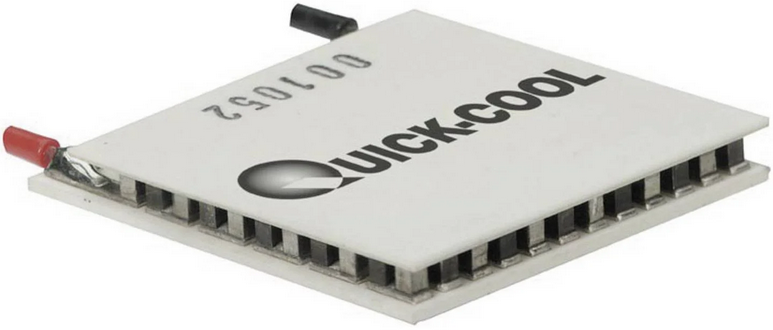
\includegraphics[scale=0.5]{98_images/peltier_modul.PNG}
    \caption{Abgebildet ist ein TEC der Marke Quick-Cool.}
    \label{fig:peltierelement}
\end{figure}

\begin{figure}[H]
    \centering
    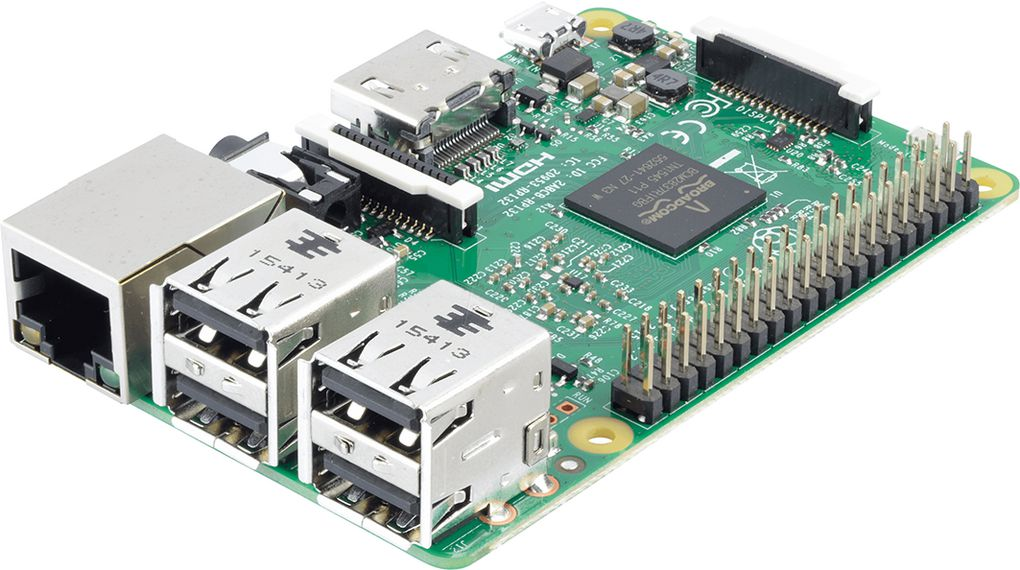
\includegraphics[scale=0.2]{98_images/raspberry_pi_version_3_b.jpg}
    \caption{Ein Raspberry PI Einplatinencomputers vom Typ Raspberry PI 3B+.}
    \label{fig:raspberry_pi}
\end{figure}

\subsection{Regelung der Thermoelektrischen Elemente (TECs)}
Optimal sollen beide TECs mit einem einzigen Treiber mit zwei Kanälen geregelt werden können. Den Verlauf der Temperaturen soll bei Möglichkeit auf einer Digitalanzeige als Graphen abgebildet werden.

\begin{figure}[H]
    \centering
    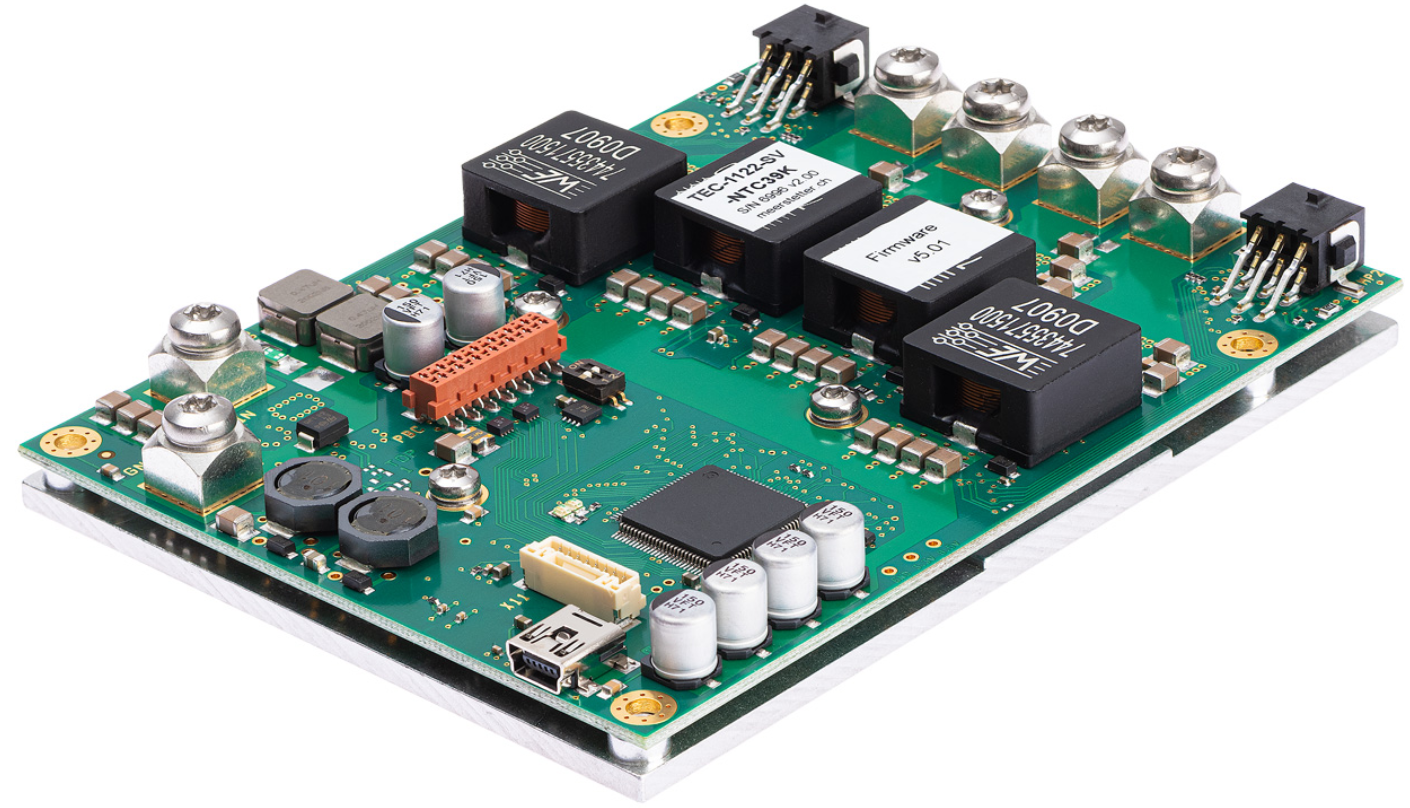
\includegraphics[scale=0.25]{98_images/tec_controller_real_isometry_meerstetter.PNG}
    \caption{Ein zwei-kanaliger TEC-Treiber vom Hersteller Meerstetter Engineering.}
    \label{fig:tec_controller_free}
\end{figure}

\subsection{Steuerung des Laserdioden-Treibers (LDD)}
Der Laserdioden-Treiber steuert die Stromzufuhr zur Pumpdiode. Dieser soll die Höhe des Stromflusses über die Steuerung erhalten. Der Stromfluss soll auf der Digitalanzeige manuell eingestellt werden können. Dafür muss eine Aus- und Eingangserweiternde Platine zum Raspberry PI angeschlossen werden, um auch analoge Signale verarbeiten zu können.
So kann der Laser ideal eingestellt werden. Die Leistung des Oszillators kann so gesteigert und durch die Steuerung die Handhabung des Lasers massiv vereinfacht werden.  % Dieser weist die Funktion auf den Stromfluss des Ausgangs über einen analogen Eingang steuern zu können.

\begin{figure}[H]
    \centering
%     %[trim={left bottom right top},clip]
    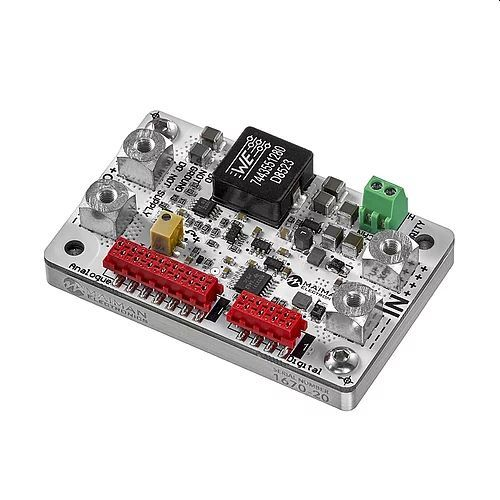
\includegraphics[scale=0.4, trim={0 30mm 0 40mm},clip]{98_images/ldd_maiman.jpg}
    \caption{Ein Laserdioden-Treiber vom Hersteller Maiman.}
    \label{fig:ldd}
\end{figure}

\subsection{Optimierung der Ausgangsleistung des Oszillators durch Justieren der Faser}
Die Ausgangsleistung des Oszillators wird stark durch die Art der Polarisation und deren Ausrichtung des Pumplasers beeinflusst. Dies hängt stark von der optischen Faser ab, in der der Pumplaser geleitet wird. Die Form der Glasfaser ist mechanisch so zu verändern, dass der ausgekoppelte Pumplaser eine möglichst optimale Form für den Oszillator aufweist. Herauszufinden ist, wie stark sich neben der Änderung der Ausrichtung der Polarisierung auch deren Form (linear, zirkular, elliptisch) verändert. Für die Anwendung in diesem Projekt wird eine möglichst horizontale und lineare Form angestrebt zu sehen in der Abb. \ref{fig:polarization_forms_directions} weiter unten.\\

\begin{figure}[H]
    \centering
    %[trim={left bottom right top},clip]
    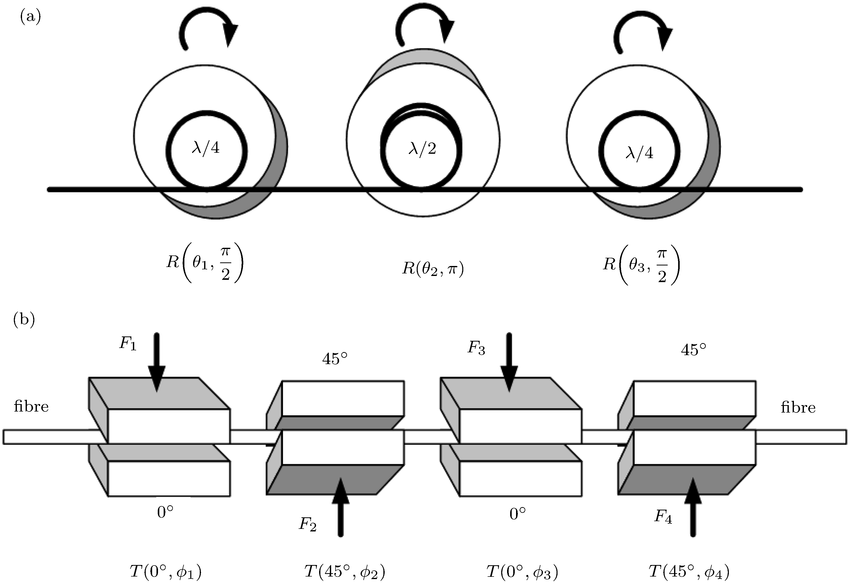
\includegraphics[scale=0.4, trim={15mm 125mm 0 0},clip]{98_images/laser_plarizationcontroller.png}
    \caption{Prinzip eines Polarizationskontrollers für die Justierung des Lasers in der Glasfaser (Auf der Abbildung in fett-schwarz)}
    \label{fig:polarizationcontroller}
\end{figure}

\begin{figure}[H]
    \centering
    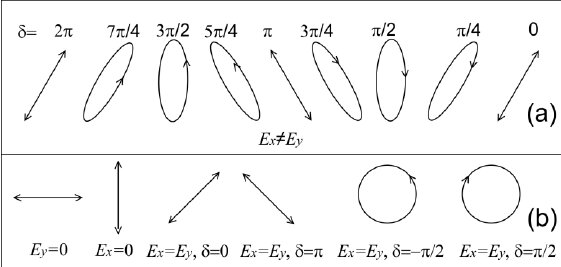
\includegraphics[scale=0.5, trim={5mm 10mm 0 14mm},clip]{98_images/laser_polarization_forms_directions.jpg}
    \caption{Abgebildet sind verschiedene Formen und Ausrichtungen der Polarisation eines Laserstrahls in Richtung seiner Achse. Abgebildet sind lineare, elliptische und zirkulare Formen der Polarisation.}
    \label{fig:polarization_forms_directions}
\end{figure}

\subsection{Weiteres}
Sollte der Zeitrahmen des Projektes dies erlauben, so ist die konzeptionelle Konstruktion des Gehäuses für den Laseraufbau zu erstellen. [14]